\section{Method}

We started with identification of common patterns occurring in the sample sequences that we would use to test our eye tracker on. Based on these patterns we have then formed our ideas of how should the software perform the detection. The patterns we have observed are as follows:

\begin{enumerate}

\item All sequences are taken with an IR camera, therefore the image has low chromaticity, but high luminance response. Therefore color could not be used to detect the eye, only the intensity.
\item Similarly, all sequences have resolution of 640x480 pixels, as a result of being taken with a web cam.
\item In all sequences there is one and only one eye, even though blinks can occur, so no pupil is visible
\item All sequences are shorter than 30 seconds

\end{enumerate}

We have built our eye tracker with these assumptions, so if any of them is broken (apart from 4.), our software will probably struggle to give a correct result. Another consideration we have made is that the performance is not the objective at this stage, so we have preferred solutions that are correct and complete over solutions that are fast. That being said, the software could still be optimized for performance and lower memory footprint removing a lot of repetition of the same calculations and code that has been introduced to enable parametrization of our partial functions.

During our work we were looking for solutions that would require as few parameters as possible, ideally none. This has led us to using k-means to obtain parameters for thresholding, which are quite volatile and trade them for parameters to k-means, which are far less volatile. In fact we have been able to use the single value for all sequences.

Similarly we have looked at all improvements to the algorithm by comparing the results of our test (Described in Section 3 Results) to the best previously achieved result. If the proposed improvement was better in all cases (increased the number of correct detections) then it was accepted, if this was not the case, it was rejected.

The following subsections detail the concrete methods we have applied to get pupil, iris and glints from the images. All of them work on grayscale images.

\subsection{Pupil Detection}
For pupil detection we start off by computing k-means for a downsized grayscale image. K-means algorithm iteratively partitions all the pixels into k clusters, where each pixel belongs to a cluster with the nearest mean. In praxis this means that it will separate different levels of gray into separate regions. You can see an example of k-means clustering on Figure \ref{fig:kmeans}.

\begin{figure}[h!]
\centering
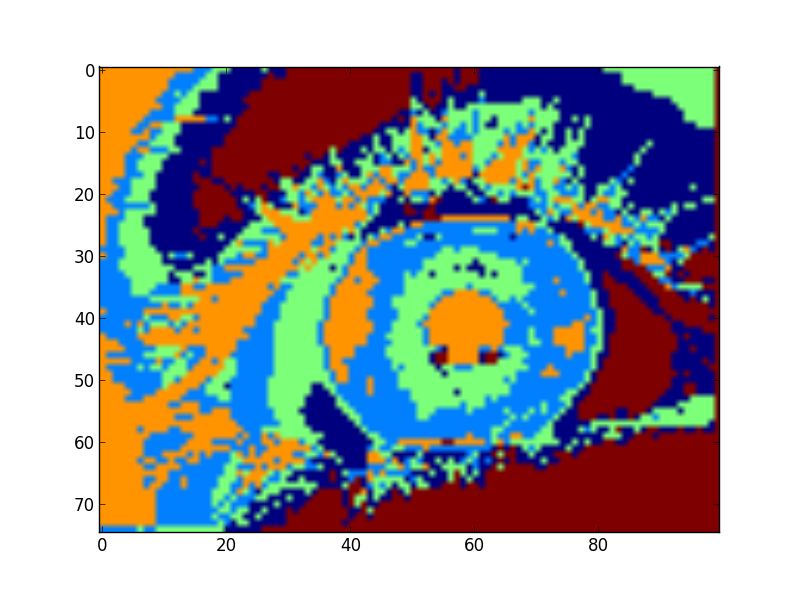
\includegraphics[width=\columnwidth]{Handin1/images/k-means.png}
\caption{k-means clustering}
\label{fig:kmeans}
\end{figure}

Since the pupil is usually very dark, it is (in most cases) safe to assume that it will be contained in the first cluster (the darkest). Therefore k-means can be used in this way to circumvent the need of setting threshold values for the thresholding function that comes next. Instead of a pre-chosen threshold we simply use the value of the first cluster. That ensures that the threshold will be set to contain the darkest values in the image (and by extension likely the pupil). The thresholded image obtained using the k-means from Figure \ref{fig:kmeans} can be seen in Figure \ref{subfig:thresh}. 

\begin{figure}[h!]
	\centering
	
	\begin{subfigure}[b]{0.5\textwidth}
		\centering
		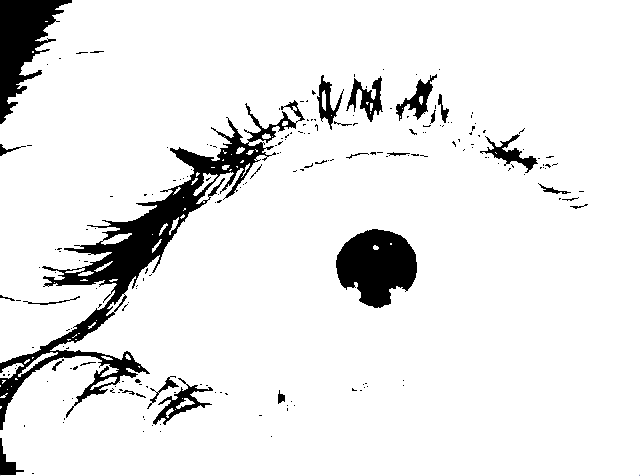
\includegraphics[width=\textwidth]{Handin1/images/thresh.png}
		\caption{After Thresholding}
		\label{subfig:thresh}
	\end{subfigure}%
	~
	\begin{subfigure}[b]{0.5\textwidth}
		\centering
		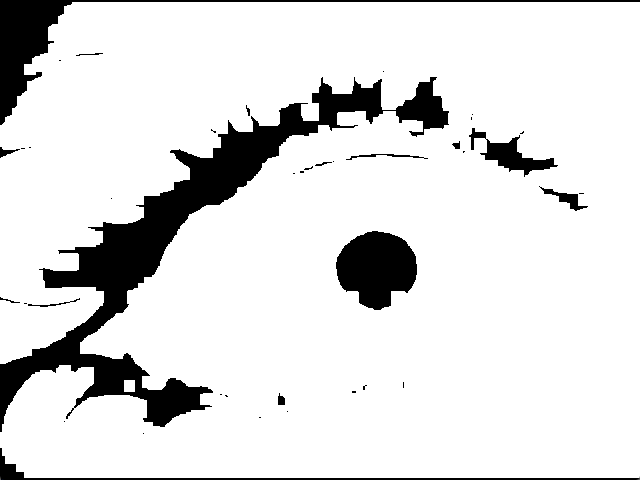
\includegraphics[width=\textwidth]{Handin1/images/open.png}
		\caption{After Opening}
		\label{subfig:open}
	\end{subfigure}
	
	\caption{Thresholding and Opening}
	\label{fig:threshopen}
\end{figure}

After thesholding we perform opening. Opening is a morphological operation that consists of performing erosion followed by dilation. This cleans up the image, removing noise and speckles. You can see this in the Figure \ref{subfig:open}.

This gives us an image that is well suited for blob analysis. We perform this in two steps. First we remove all blobs which are bigger than 30\% of the image area or smaller than 0.2\% of the entire image. This removes blobs that are most likely not pupil. Second fit an ellipse to the contour and then we compare the ratio between the two radii of that ellipse. That removes all matches that are too elliptical. The pupil is usually more like a circle, but can be slightly elliptical when the user is looking to the side.

The last step we perform is ordering, we order all detected ellipses by increasing extend. This ensures that the most contained blobs come first. In most cases this should prioritize well contained blobs (such as the pupil) over false positives, and all the other detection functions just take the first result from pupil detection.

We have also implemented a failsafe mechanism, that, in absence of any pupils detected, can iteratively call the getPupils() function with lower values of k, which results in better performance in sequences with high contrast. In particular in sequence 8 this change alone has improved the detection rate from 0\% to 62.5\% in the testing frames.

\subsection{Iris Detection}

For iris detection we start with the position of the pupil detected previously. First we filter the image using the Sobel filter. We then use the filtered image to calculate orientation (Figure \ref{subfig:quiver}) and magnitude (Figure \ref{subfig:magnitude}) of the gradient image. 

\begin{figure}[h!]
	\centering
	
	\begin{subfigure}[b]{0.5\textwidth}
		\centering
		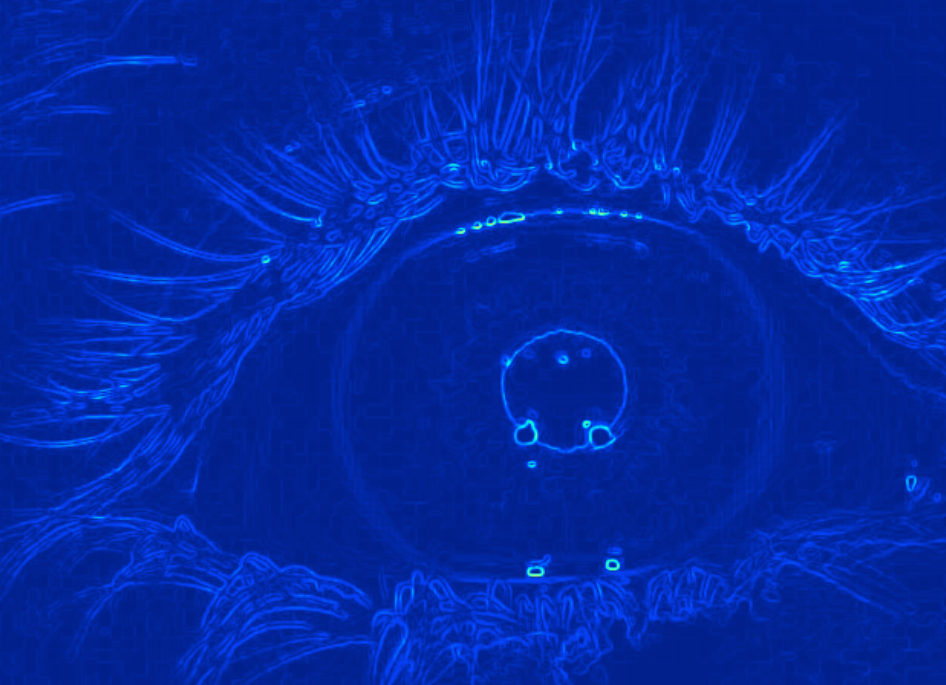
\includegraphics[width=\textwidth]{Handin1/images/magnitude.png}
		\caption{Magnitude}
		\label{subfig:magnitude}
	\end{subfigure}%
	~
	\begin{subfigure}[b]{0.5\textwidth}
		\centering
		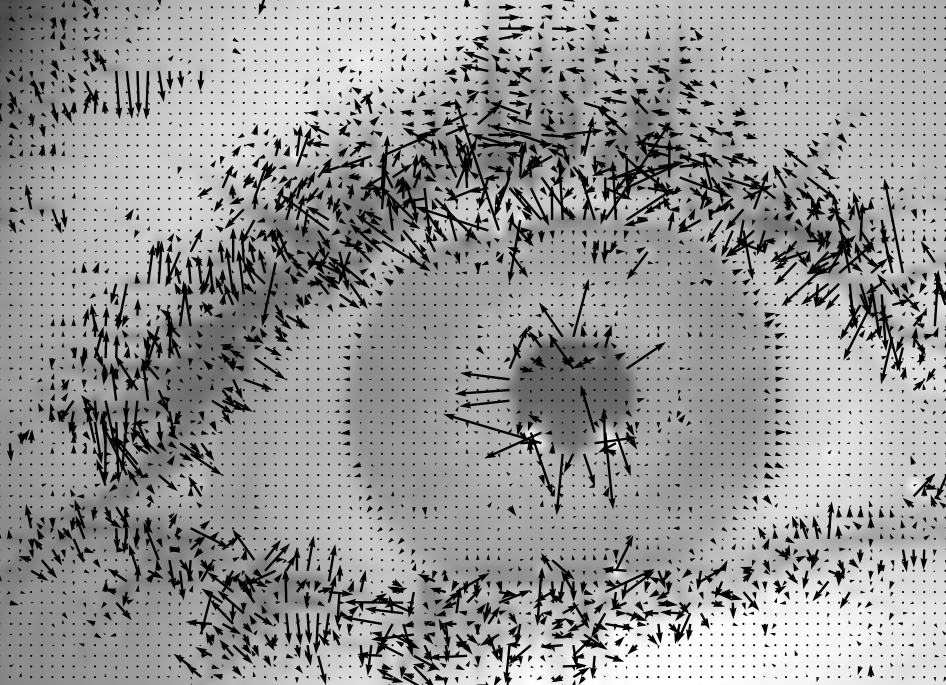
\includegraphics[width=\textwidth]{Handin1/images/quiver.png}
		\caption{Orientation}
		\label{subfig:quiver}
	\end{subfigure}
	
	\caption{Gradient Image: Magnitude and Orientation}
\end{figure}

We then use the orientation and magnitude data to estimate the iris radius. We assume that the center of iris will be the same as the center of pupil, so we sample the circle defined by pupil on 30 locations and consider lines that originate between the center of the pupil and end at a distance 5x greater than the radius of the pupil. See Figure \ref{subfig:iris_samples} for reference, samples are represented as bright green lines. 
Also in the Figure \ref{subfig:iris_samples} we can see points where sample values for orientation and magnitude correspond to the right values, and therefore are potential candidates for iris boundary. These points are represented as cyan circles in the image. The corresponding magnitude has to be greater than 15 and orientation can be no more than  5 either way from the orientation of the sample line. For each of these points we record the distance from the pupil centre, if more than one point votes for the same radius, we increment the count for that radius. At the end of this process we take the radius with most votes and proclaim it the iris boundary (Shown as a purple circle in Figure \ref{subfig:iris_estimation}).

\begin{figure}[h!]
	\centering
	
	\begin{subfigure}[b]{0.5\textwidth}
		\centering
		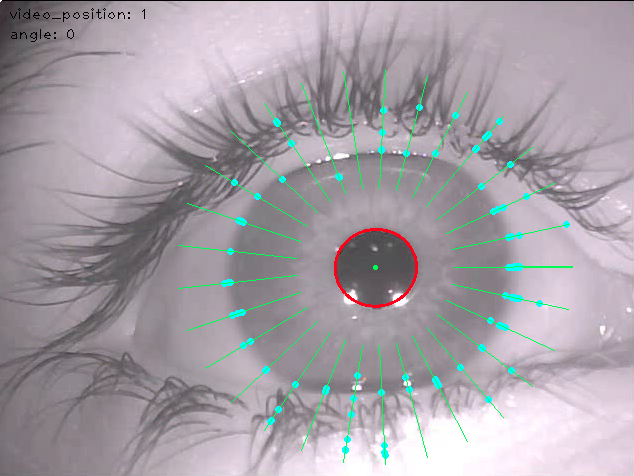
\includegraphics[width=\textwidth]{Handin1/images/iris_samples.png}
		\caption{Samples}
		\label{subfig:iris_samples}
	\end{subfigure}%
	~
	\begin{subfigure}[b]{0.5\textwidth}
		\centering
		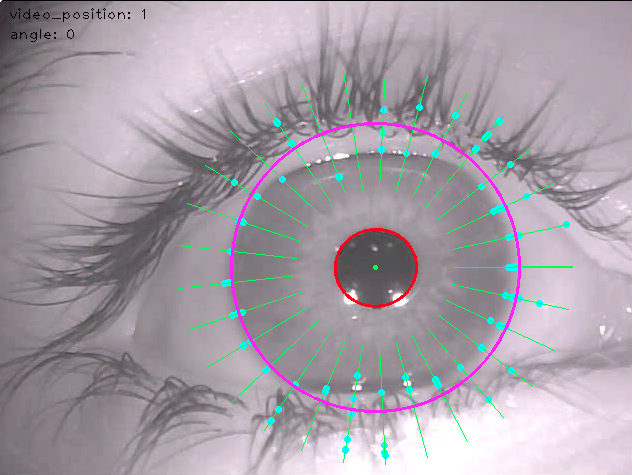
\includegraphics[width=\textwidth]{Handin1/images/iris_estimation.png}
		\caption{Estimation}
		\label{subfig:iris_estimation}
	\end{subfigure}
	
	\caption{Iris Estimation}
\end{figure}

Iris detection works a bit differently than pupil and glint detection in that it works with the assumption that the pupil was detected correctly and therefore there should be an iris to be found. So the detector just counts different votes for individual circle radii and picks the highest one. Of course the worst case for this is when pupil has been mis-detected and there is at least one corresponding orientation and magnitude for one of the 30 sample lines taken, which is highly probable. In this case the iris will be detected on this radius, even though there is only one vote.


\subsection{Glint Detection}

Glint detection is in principle very similar to pupil detection, first we compute k-means to a downsized grayscale image. Since the glint can be considered a flash of light in the eye, we assume that this will the brightest point with the first cluster. 
Therefore, we can use k-means to set the values for the thresholding functions, which are called next. After thresholding we find blobs in the image using contours. We then reject all blobs that are bigger than 0.1\% of the total image area. This ensures that we don't count big bright areas of the image as glints, since glints are usually small. As the last filter we reject all glints that have centers outside of the iris circle which we have calculated in the previous phase. This will leave us only with the glints inside the eye and nothing else.

\begin{figure}[h!]
	\centering
	
	\begin{subfigure}[b]{0.5\textwidth}
		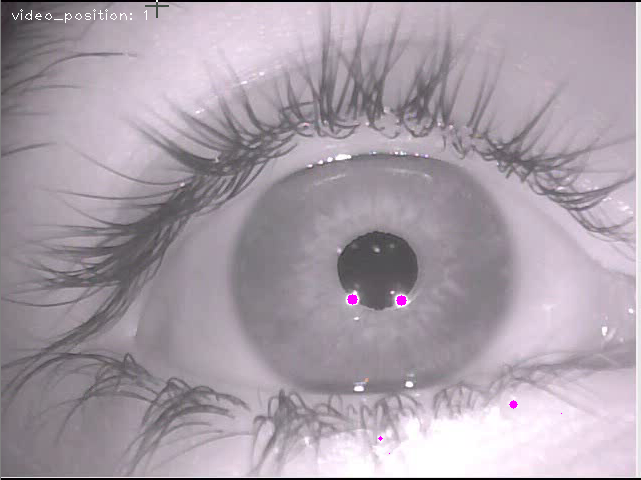
\includegraphics[width=\textwidth]{Handin1/images/glitDetection.png}
		\caption{Glint Detection}
		\label{subfig:glints}
	\end{subfigure}%
	~
	\begin{subfigure}[b]{0.5\textwidth}
		\centering
		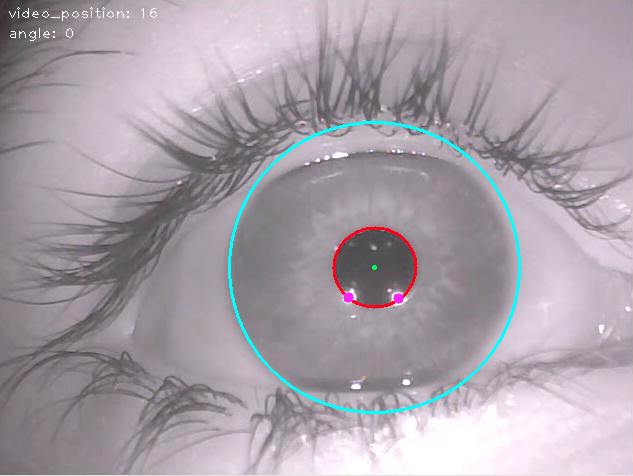
\includegraphics[width=\textwidth]{Handin1/images/final.png}
		\caption{Final Image}
		\label{subfig:final}
	\end{subfigure}
	
	\caption{Glint Detection Phase}
\end{figure}




